Ce chapitre présente les technologies utilisées, l'architecture technique, et les interfaces développées pour le système PBADS.

\section{Technologies et Architecture}

\subsection{Architecture microservices}

Notre système suit une architecture microservices moderne, séparant clairement les responsabilités entre les différents services pour garantir la scalabilité, la maintenabilité et la tolérance aux pannes.

\textbf{Composants de l'architecture :}

\begin{itemize}
    \item \textbf{Frontend (Thymeleaf) :} Interface utilisateur développée avec Thymeleaf et Chart.js
    \item \textbf{Backend (Spring Boot) :} APIs REST développées avec Spring Boot
    \item \textbf{Bases de données (PostgreSQL) :} Bases de données relationnelles avec JPA/Hibernate
    \item \textbf{Sécurité :} Authentification JWT et contrôle d'accès basé sur les rôles
    \item \textbf{Communication :} Kafka pour la messagerie asynchrone et HTTP/REST pour les appels synchrones
    \item \textbf{Machine Learning :} Python (scikit-learn) pour l'entraînement et l'inférence des modèles
    \item \textbf{IA :} Google Gemini AI pour la génération de recommandations personnalisées
\end{itemize}

\subsection{Technologies Frontend}

\subsubsection{Thymeleaf}

Thymeleaf constitue le moteur de template côté serveur pour notre interface utilisateur, offrant une intégration native avec Spring MVC.

\textbf{Composants principaux :}
\begin{itemize}
    \item \textbf{Templates :} Pages HTML avec syntaxe Thymeleaf pour le rendu dynamique
    \item \textbf{Fragments :} Composants réutilisables (navbar, footer)
    \item \textbf{Expressions :} Accès aux données du modèle et aux variables de session
    \item \textbf{Sécurité :} Intégration avec Spring Security pour la protection des routes
\end{itemize}

\subsubsection{Chart.js}

Chart.js fournit une bibliothèque de graphiques JavaScript pour la visualisation interactive des données comportementales.

\textbf{Composants utilisés :}
\begin{itemize}
    \item \textbf{Graphiques linéaires :} Visualisation des tendances comportementales dans le temps
    \item \textbf{Filtres temporels :} Filtrage par semaine, mois, année, ou toutes les données
    \item \textbf{Animations :} Transitions fluides lors du changement de filtres
    \item \textbf{Thème sombre :} Interface adaptée avec palette de couleurs personnalisée
\end{itemize}

\subsection{Technologies Backend}

\subsubsection{Spring Boot Framework}

Spring Boot constitue la base de nos APIs REST, offrant une configuration simplifiée et des fonctionnalités enterprise robustes.

\textbf{Modules Spring utilisés :}
\begin{itemize}
    \item \textbf{Spring Web :} Développement d'API REST avec annotations
    \item \textbf{Spring Security :} Gestion de la sécurité et de l'authentification
    \item \textbf{Spring Data JPA :} Abstraction de la couche de données
    \item \textbf{Spring Cloud Gateway :} Point d'entrée unique pour toutes les requêtes
    \item \textbf{Spring Cloud Eureka :} Découverte de services
    \item \textbf{Spring Cloud Config :} Configuration centralisée
    \item \textbf{Spring Cloud OpenFeign :} Client HTTP déclaratif pour la communication entre services
\end{itemize}

\subsubsection{Kafka}

Apache Kafka est utilisé comme broker de messagerie pour la communication asynchrone entre services.

\textbf{Topics utilisés :}
\begin{itemize}
    \item \texttt{data.logged.events} : Événements de données quotidiennes enregistrées
    \item \texttt{anomaly.detected.events} : Événements d'anomalies détectées
\end{itemize}

\subsubsection{PostgreSQL Database}

PostgreSQL a été choisi comme base de données relationnelle pour sa robustesse et ses performances.

\textbf{Bases de données :}
\begin{itemize}
    \item \texttt{pbads\_auth} : Données d'authentification et utilisateurs
    \item \texttt{pbads\_data} : Données quotidiennes des utilisateurs
    \item \texttt{pbads\_alerts} : Alertes générées
\end{itemize}

\subsection{Machine Learning}

\subsubsection{scikit-learn}

scikit-learn est utilisé pour l'entraînement et l'inférence des modèles de détection d'anomalies.

\textbf{Algorithmes utilisés :}
\begin{itemize}
    \item \textbf{Isolation Forest :} Algorithme principal pour la détection d'anomalies
    \item \textbf{One-Class SVM :} Algorithme alternatif avec noyau RBF
\end{itemize}

\subsubsection{MLflow}

MLflow est utilisé pour le suivi des expériences ML et le versioning des modèles.

\section{Interfaces Utilisateur}

Cette section présente les interfaces développées pour les utilisateurs et les administrateurs du système PBADS.

\subsection{Vue Utilisateur}

\subsubsection{Page d'inscription}

\begin{figure}[H]
    \centering
    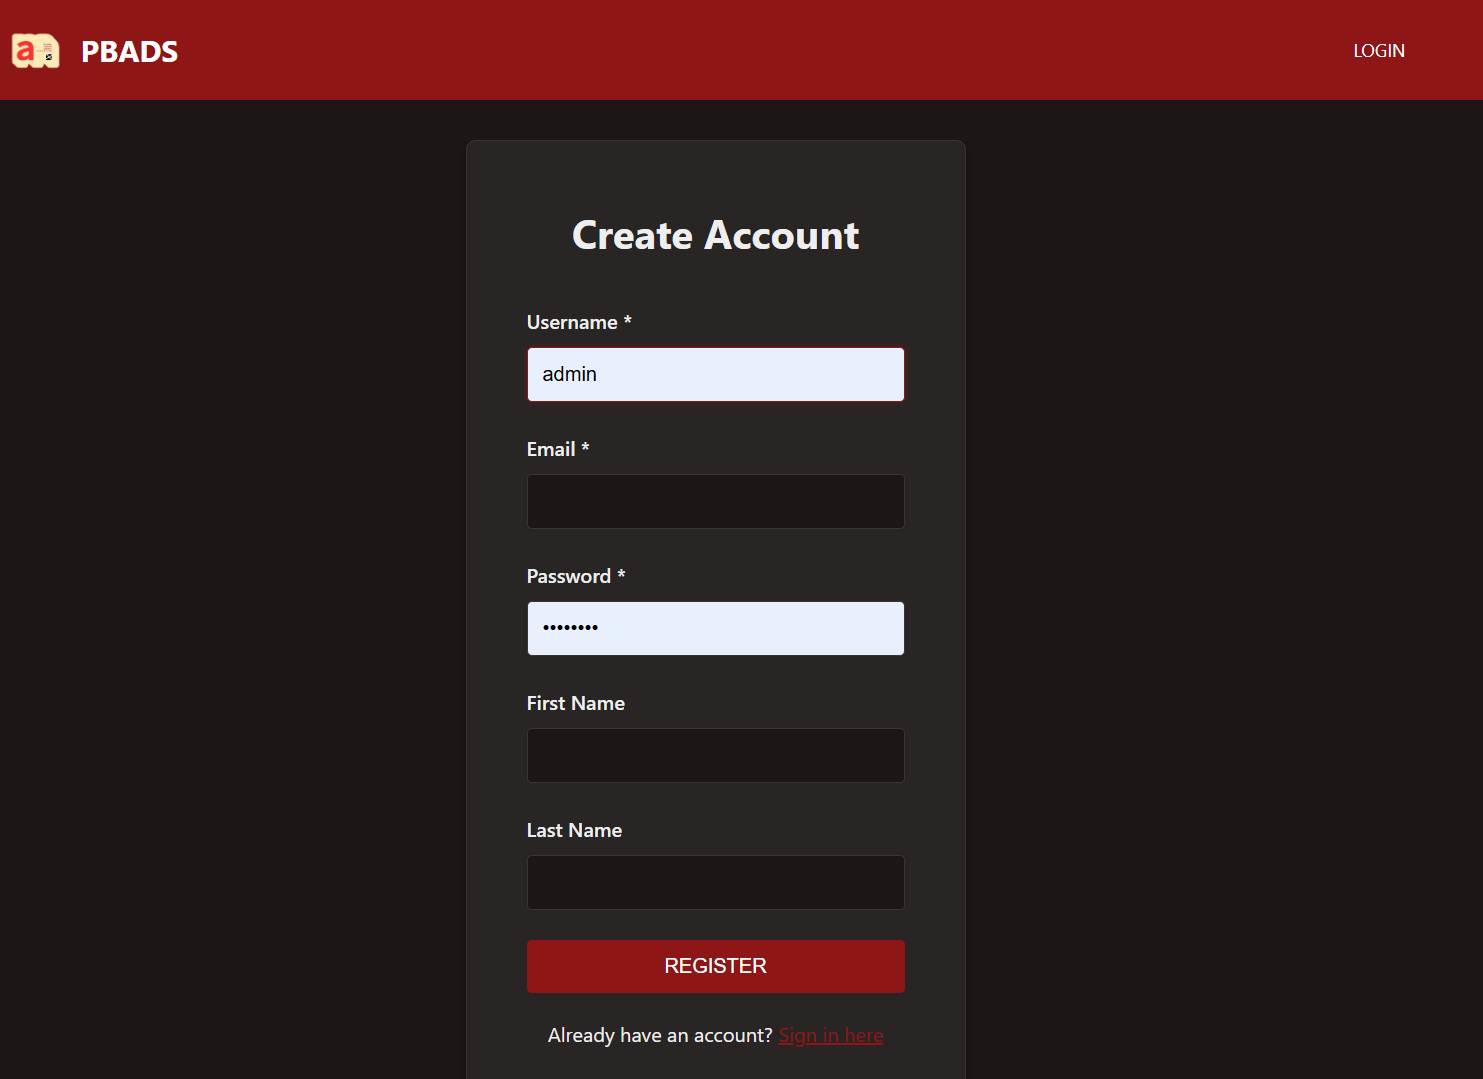
\includegraphics[width=\textwidth]{Figures/pbadsuser/userregisterpage.png}
    \caption{Page d'inscription - Création de compte utilisateur}
    \label{fig:user-register}
\end{figure}

Cette interface permet aux nouveaux utilisateurs de créer un compte dans le système PBADS. Le formulaire collecte les informations essentielles : nom d'utilisateur, email, mot de passe, et prénom/nom. La page utilise un thème sombre moderne avec une navigation simplifiée (seul le lien "LOGIN" est visible pour les utilisateurs non authentifiés).

\subsubsection{Page de connexion}

\begin{figure}[H]
    \centering
    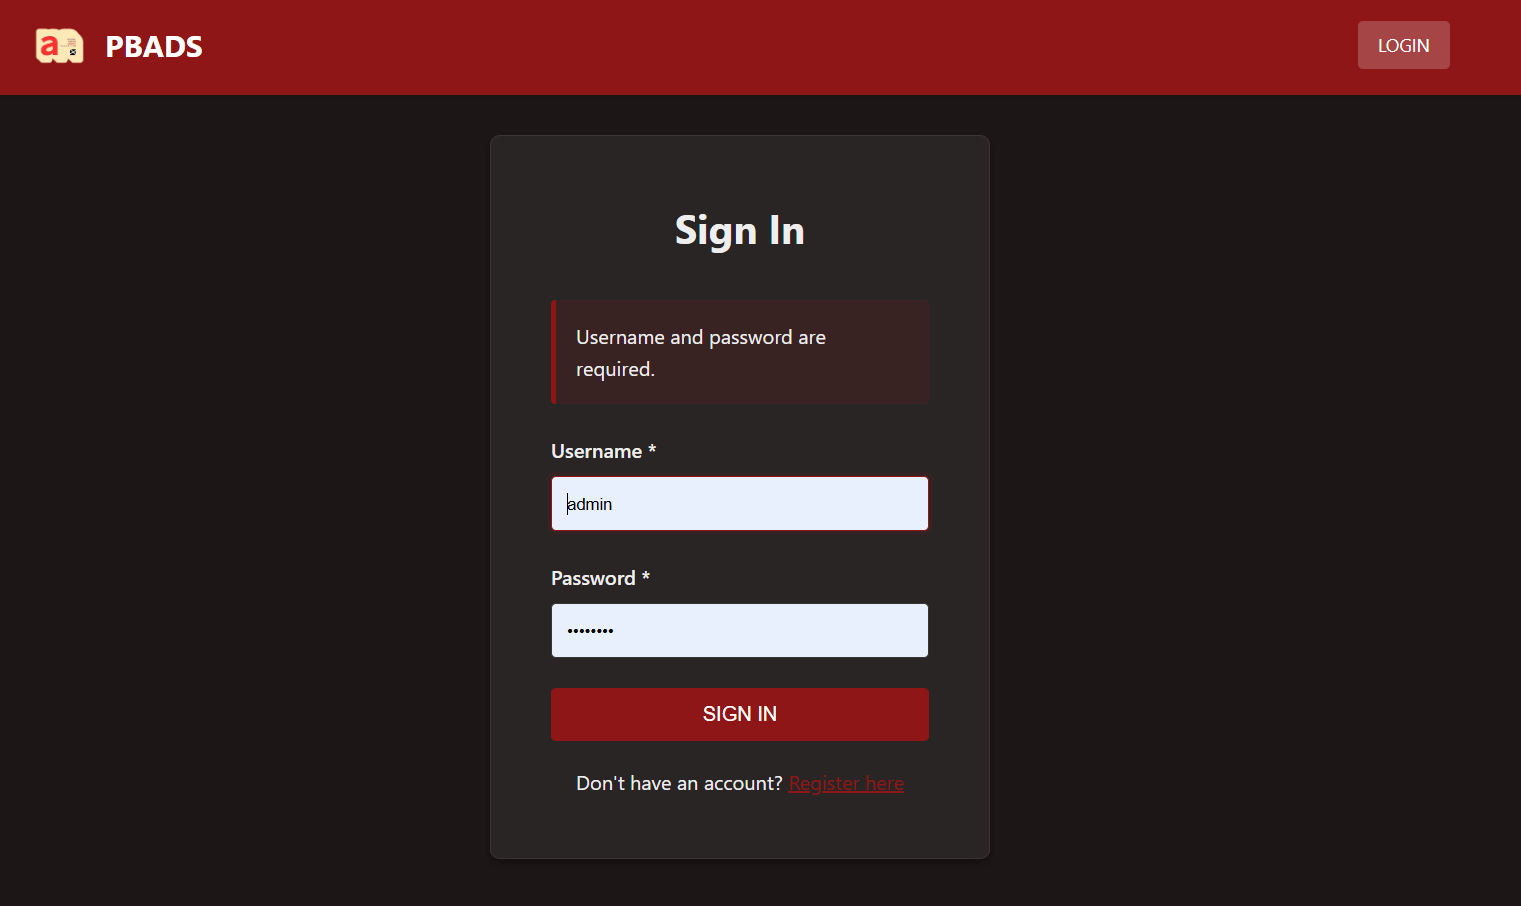
\includegraphics[width=\textwidth]{Figures/pbadsuser/usersigninpage.png}
    \caption{Page de connexion - Authentification utilisateur}
    \label{fig:user-signin}
\end{figure}

Cette interface permet aux utilisateurs de se connecter au système avec leurs identifiants (nom d'utilisateur et mot de passe). La page suit le même thème sombre cohérent avec le reste de l'application et offre un accès rapide à la page d'inscription pour les nouveaux utilisateurs.

\subsubsection{Tableau de bord - Graphiques}

\begin{figure}[H]
    \centering
    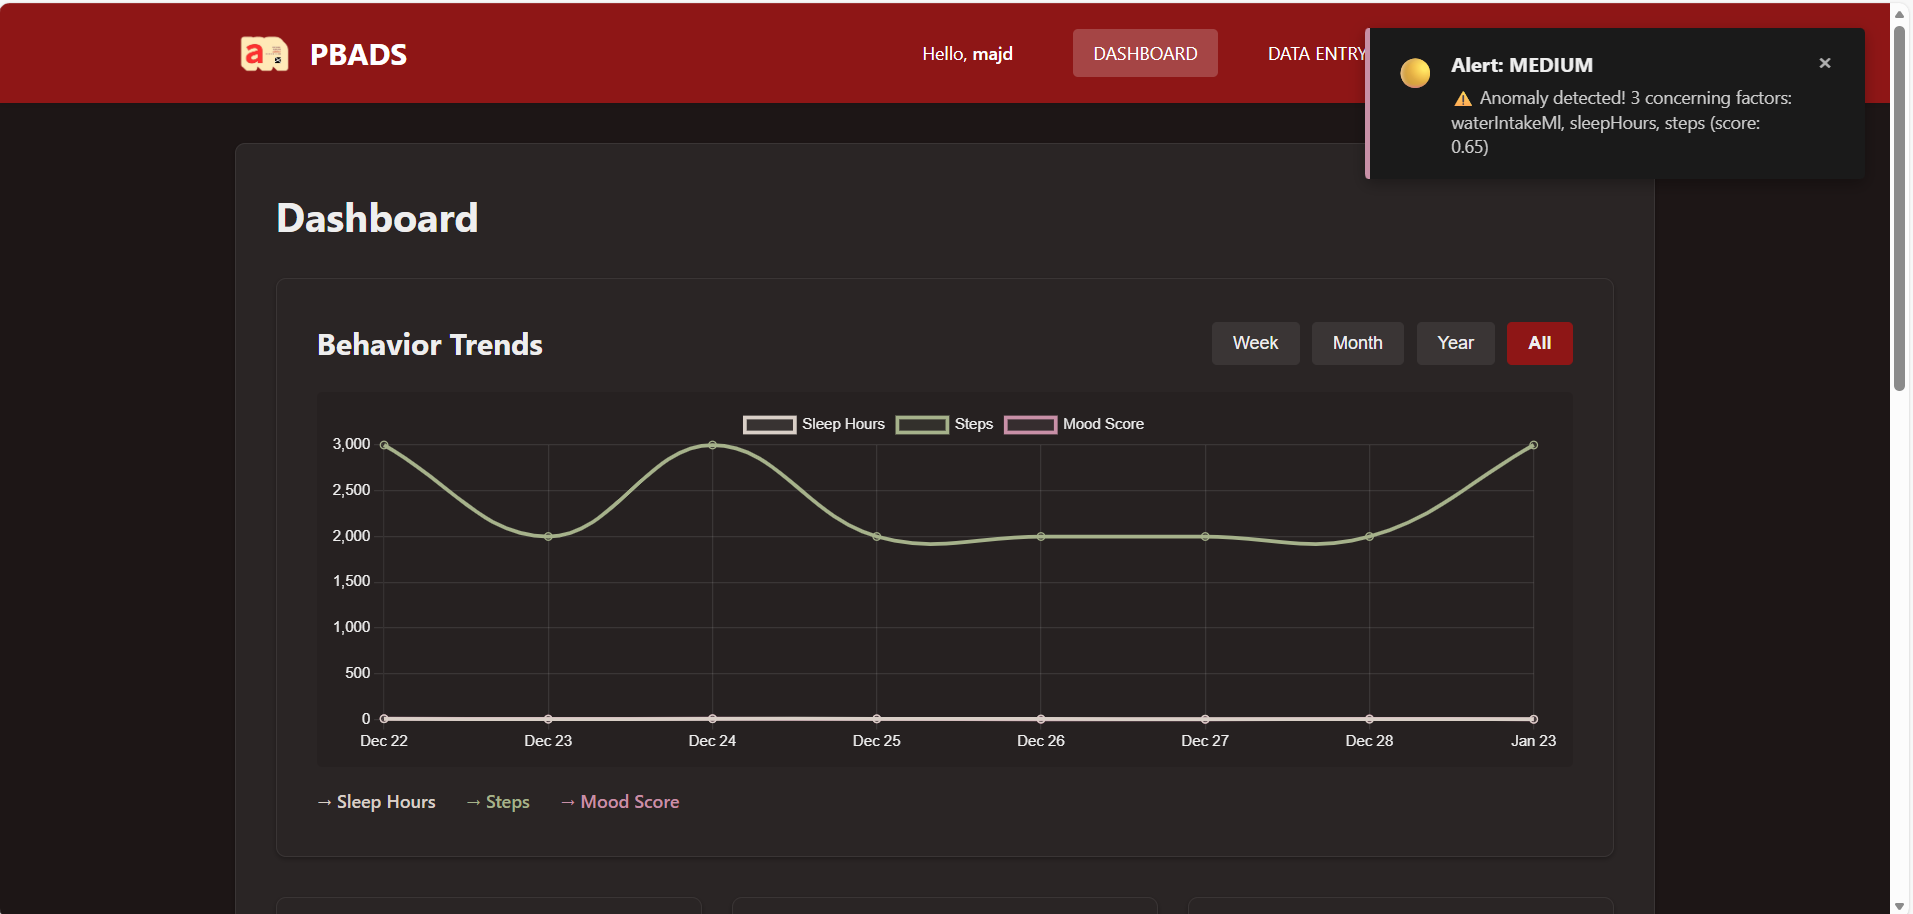
\includegraphics[width=\textwidth]{Figures/pbadsuser/userdashboardgraph.png}
    \caption{Tableau de bord - Visualisation des tendances comportementales}
    \label{fig:user-dashboard-graph}
\end{figure}

Cette interface constitue le cœur du système PBADS, présentant une visualisation interactive des données comportementales de l'utilisateur. Le tableau de bord inclut :

\begin{itemize}
    \item \textbf{Graphique des tendances comportementales :} Visualisation des données quotidiennes avec Chart.js
    \item \textbf{Filtres temporels :} Boutons pour filtrer par semaine, mois, année, ou toutes les données
    \item \textbf{Statistiques résumées :} Vue d'ensemble des métriques clés (sommeil moyen, steps moyens, etc.)
    \item \textbf{Thème sombre :} Interface moderne avec palette de couleurs personnalisée (\#1a1a1a, \#2d2d2d, \#8E1616)
\end{itemize}

\subsubsection{Tableau de bord - Alertes et Recommandations}

\begin{figure}[H]
    \centering
    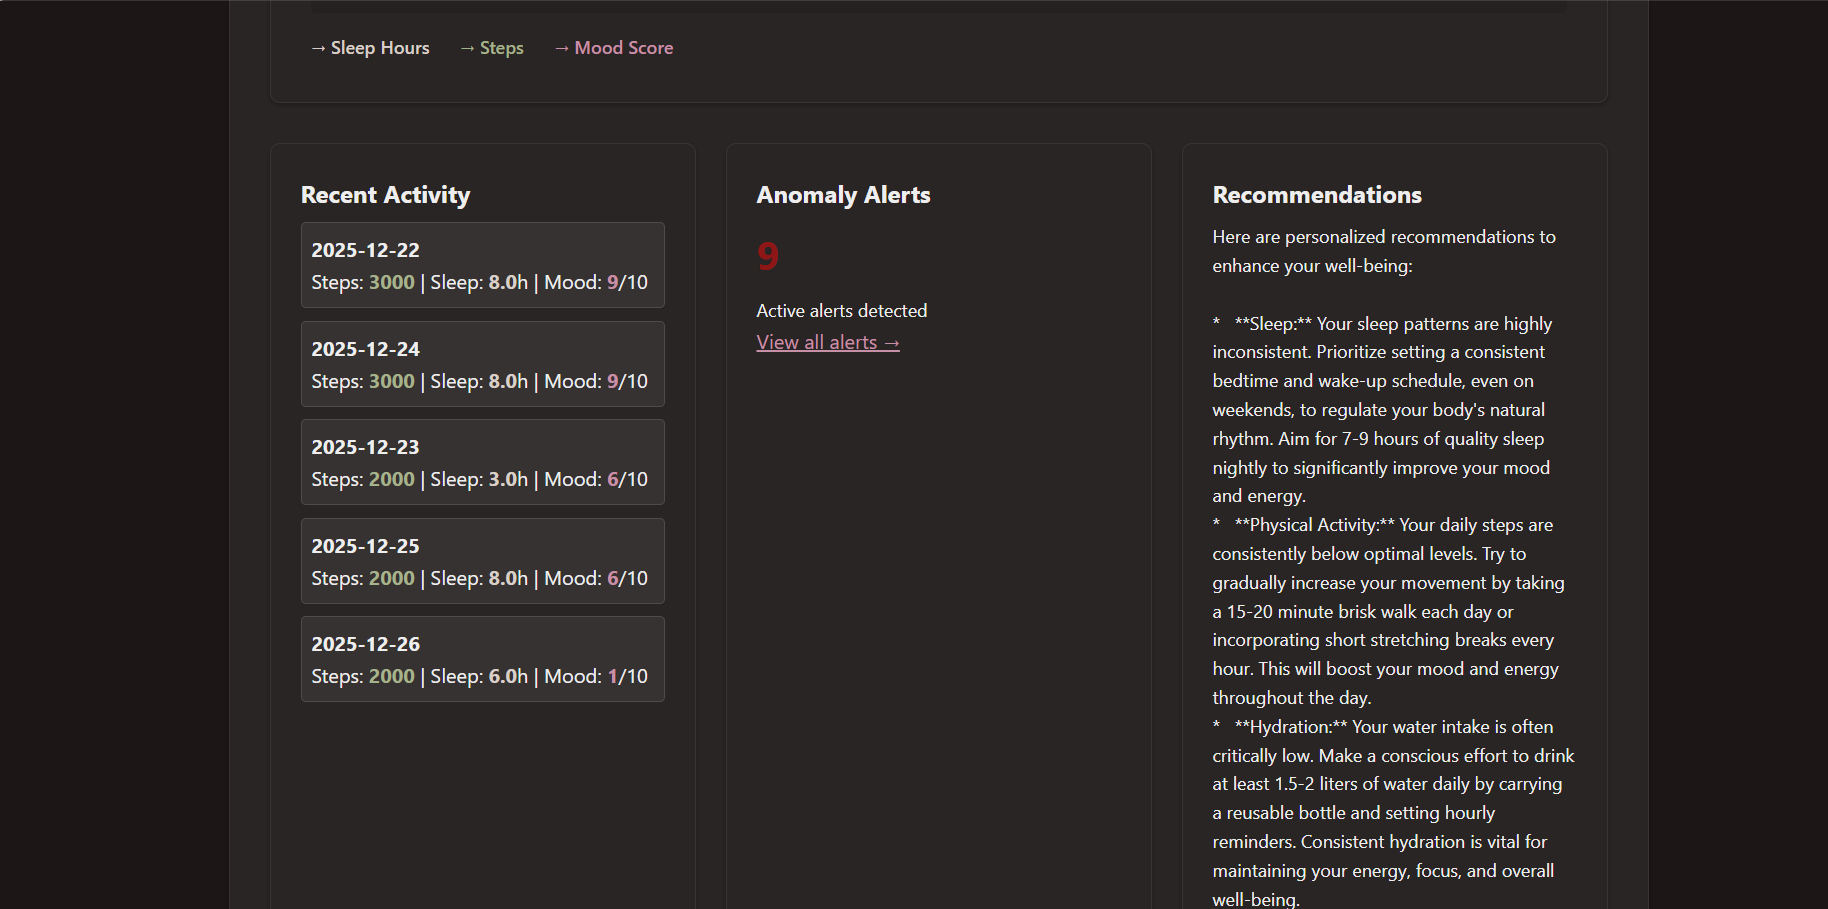
\includegraphics[width=\textwidth]{Figures/pbadsuser/userdashboardalertsandrecommandation.png}
    \caption{Tableau de bord - Alertes et recommandations IA}
    \label{fig:user-dashboard-alerts}
\end{figure}

Cette section du tableau de bord présente les alertes générées et les recommandations personnalisées. L'interface affiche :

\begin{itemize}
    \item \textbf{Alertes récentes :} Liste des alertes avec niveaux de sévérité (HIGH, MEDIUM, LOW)
    \item \textbf{Recommandations IA :} Suggestions personnalisées générées par Google Gemini AI
    \item \textbf{Badges de statut :} Indicateurs visuels pour les niveaux d'alerte
    \item \textbf{Design cohérent :} Intégration harmonieuse avec le thème sombre du tableau de bord
\end{itemize}

\subsubsection{Saisie de données quotidiennes}

\begin{figure}[H]
    \centering
    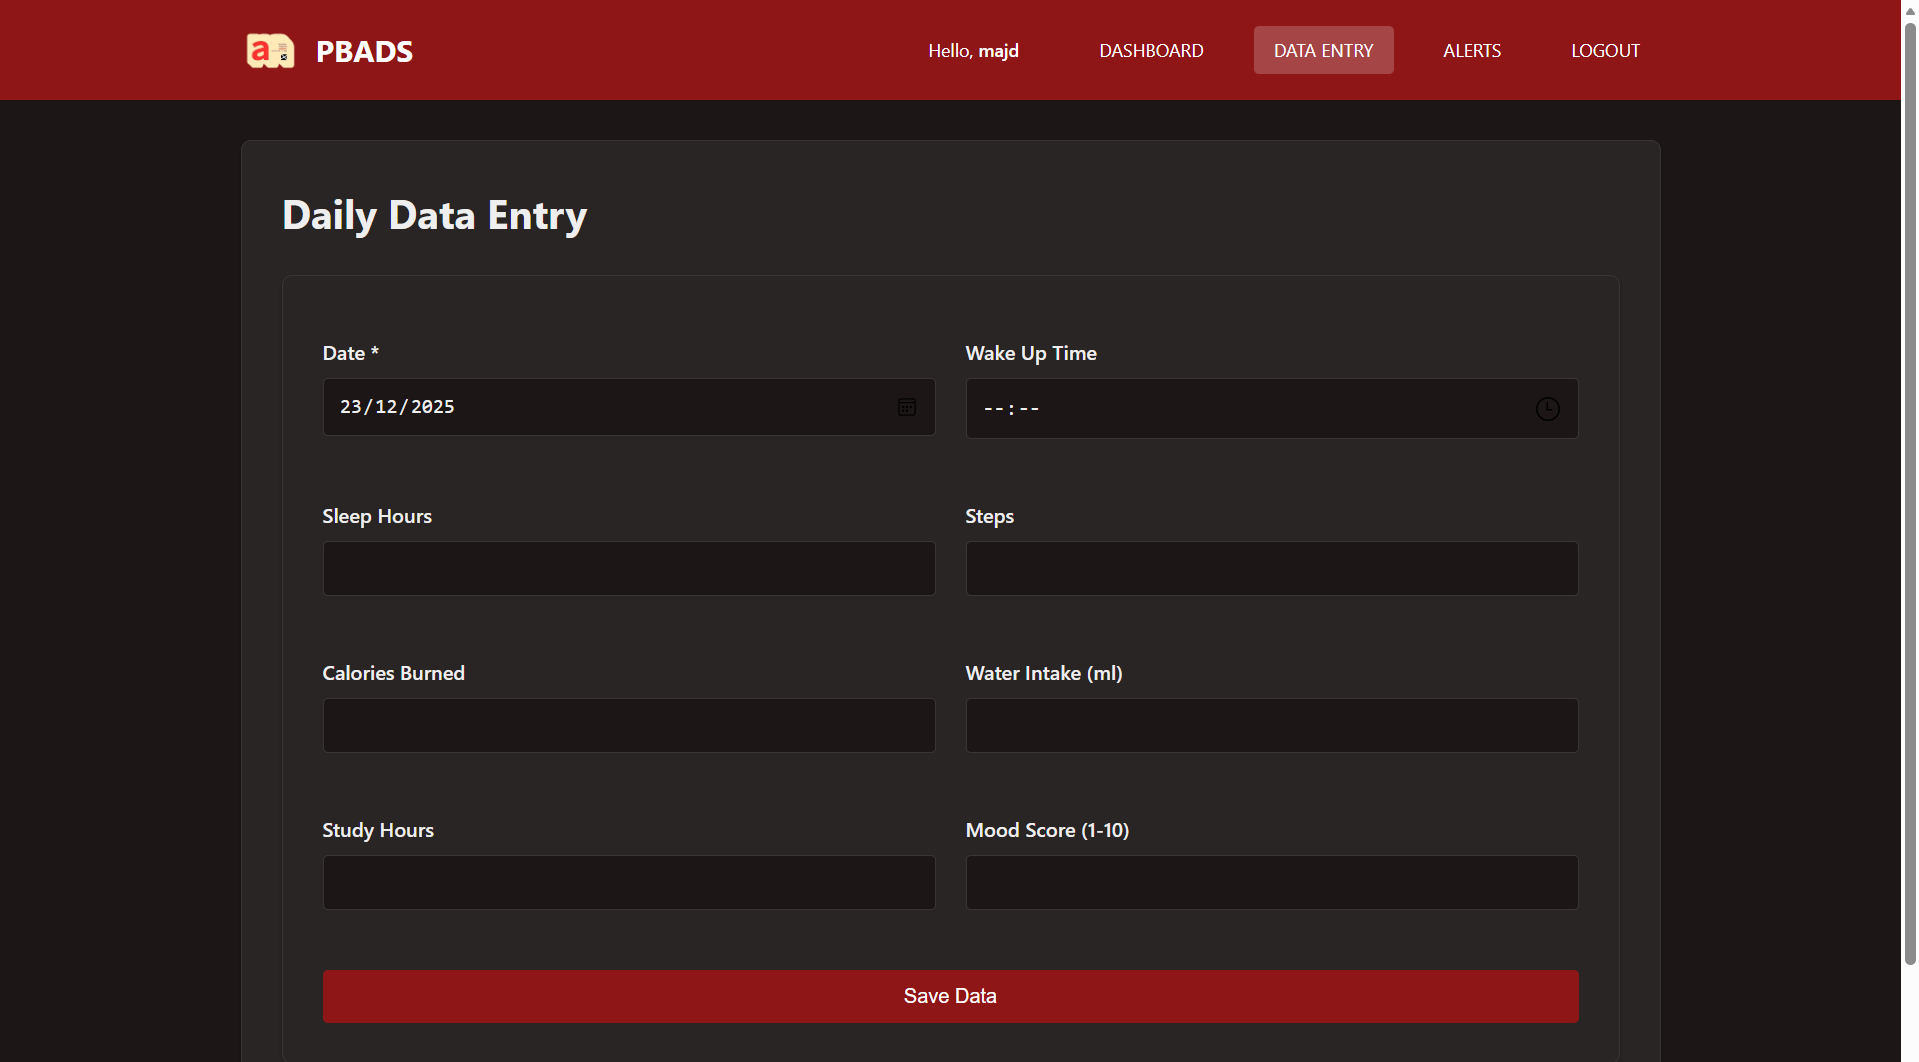
\includegraphics[width=\textwidth]{Figures/pbadsuser/userdataentry.png}
    \caption{Formulaire de saisie des données quotidiennes}
    \label{fig:user-data-entry}
\end{figure}

Cette interface permet aux utilisateurs de saisir leurs données quotidiennes de manière structurée. Le formulaire inclut :

\begin{itemize}
    \item \textbf{Date :} Sélection de la date pour laquelle les données sont enregistrées
    \item \textbf{Heure de réveil :} Champ pour l'heure de réveil
    \item \textbf{Heures de sommeil :} Nombre d'heures de sommeil
    \item \textbf{Steps :} Nombre de pas effectués dans la journée
    \item \textbf{Calories brûlées :} Nombre de calories brûlées
    \item \textbf{Consommation d'eau :} Quantité d'eau consommée en millilitres
    \item \textbf{Heures d'étude :} Temps consacré à l'étude
    \item \textbf{Score d'humeur :} Évaluation de l'humeur sur une échelle de 1 à 10
\end{itemize}

Le formulaire utilise une validation côté client et serveur pour garantir l'intégrité des données.

\subsubsection{Notification push d'alerte}

\begin{figure}[H]
    \centering
    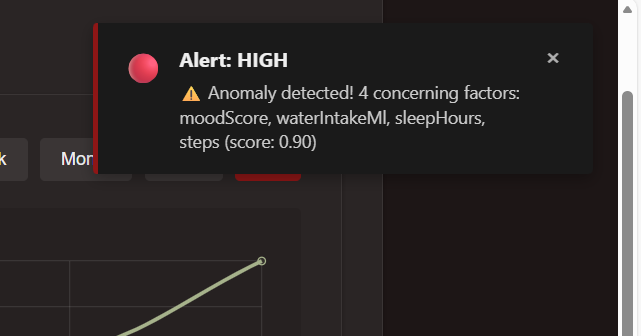
\includegraphics[width=\textwidth]{Figures/pbadsuser/userpushalert.png}
    \caption{Notification push - Alerte d'anomalie détectée}
    \label{fig:user-push-alert}
\end{figure}

Cette interface illustre le système de notifications push (toast) qui alerte les utilisateurs en temps réel lorsqu'une nouvelle anomalie est détectée. Les caractéristiques incluent :

\begin{itemize}
    \item \textbf{Notification éphémère :} Affichage temporaire en haut à droite de l'écran
    \item \textbf{Niveaux de sévérité :} Couleurs différentes selon le niveau (HIGH, MEDIUM, LOW)
    \item \textbf{Message informatif :} Description de l'anomalie détectée
    \item \textbf{Bouton de fermeture :} Possibilité de fermer manuellement la notification
    \item \textbf{Animation :} Transitions fluides pour l'apparition et la disparition
\end{itemize}

Le système poll le service d'alertes toutes les 5 secondes pour détecter les nouvelles alertes et afficher les notifications automatiquement.

\subsubsection{Page des alertes}

\begin{figure}[H]
    \centering
    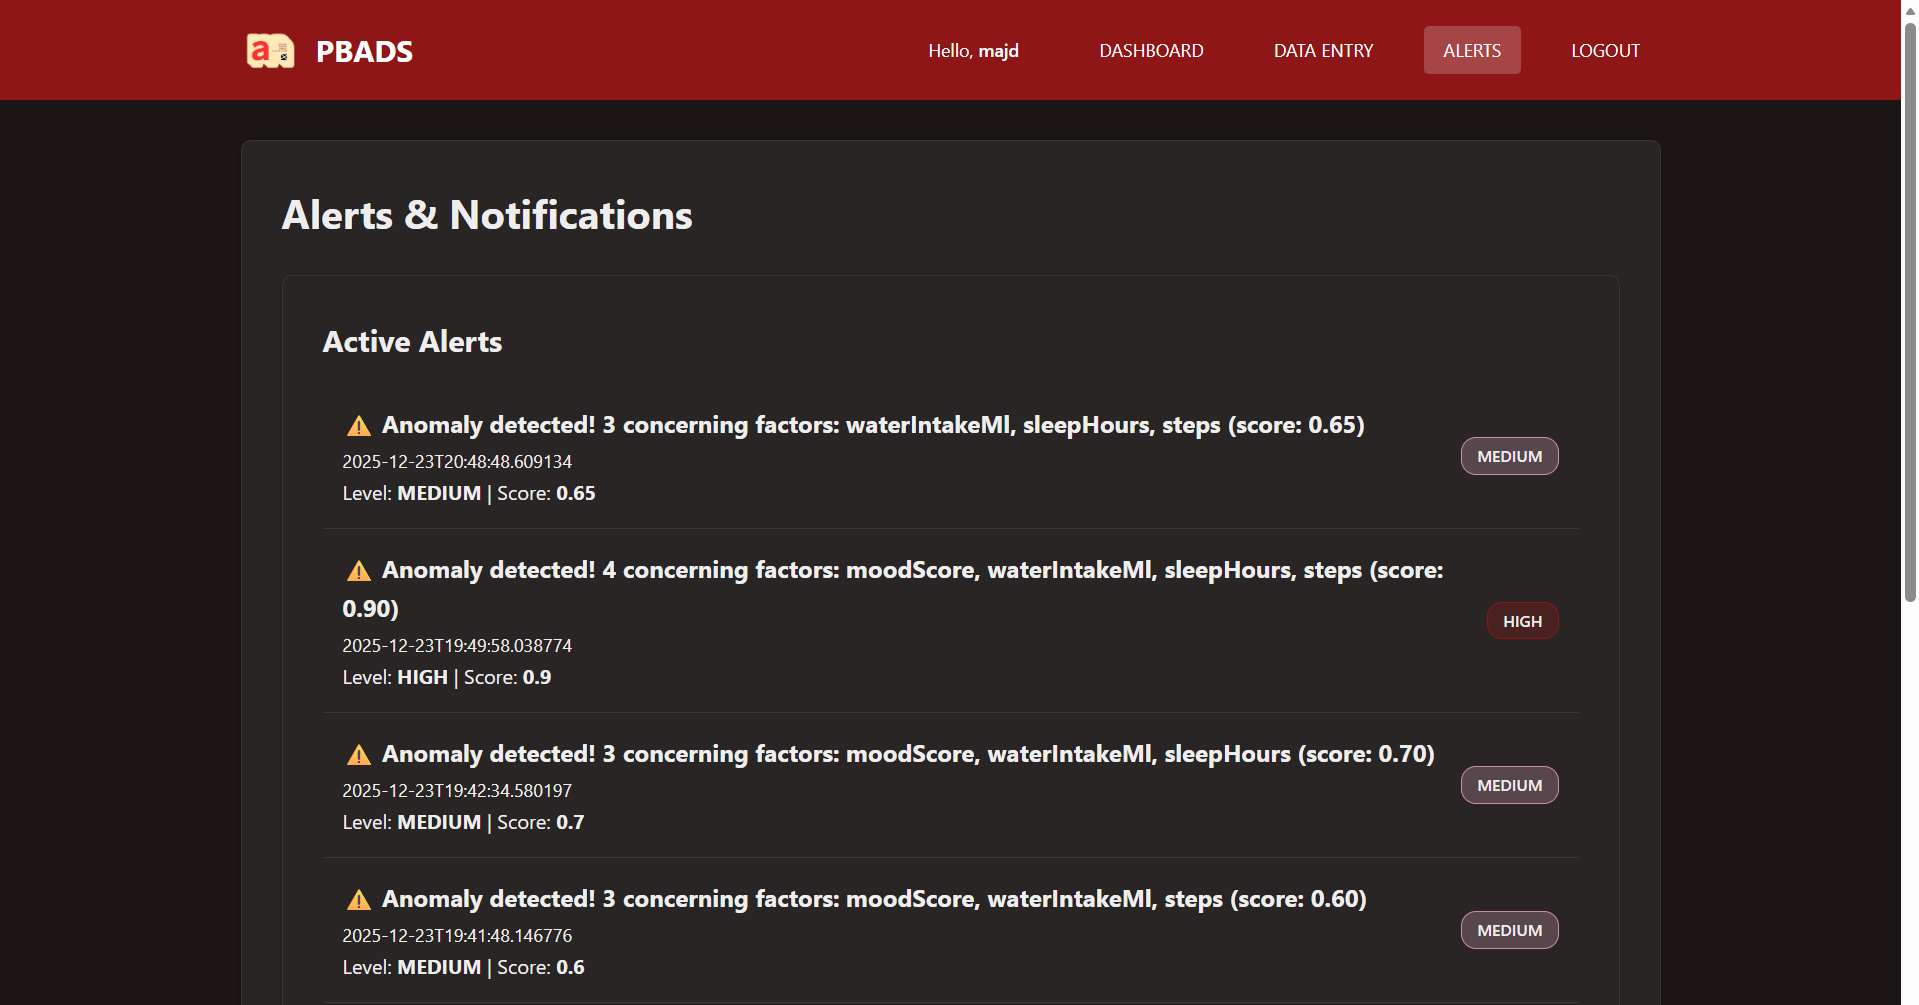
\includegraphics[width=\textwidth]{Figures/pbadsuser/useralertpage.png}
    \caption{Page de consultation des alertes}
    \label{fig:user-alert-page}
\end{figure}

Cette interface permet aux utilisateurs de consulter toutes leurs alertes de manière organisée. La page affiche :

\begin{itemize}
    \item \textbf{Liste complète des alertes :} Toutes les alertes générées pour l'utilisateur
    \item \textbf{Informations détaillées :} Date, score d'anomalie, niveau, message
    \item \textbf{Statut des alertes :} Indicateurs visuels pour ACTIVE, ACKNOWLEDGED, RESOLVED
    \item \textbf{Organisation temporelle :} Alertes triées par date (plus récentes en premier)
    \item \textbf{Design cohérent :} Thème sombre avec badges colorés pour les niveaux de sévérité
\end{itemize}

\subsection{Vue Administrateur}

\subsubsection{Gestion des utilisateurs}

\begin{figure}[H]
    \centering
    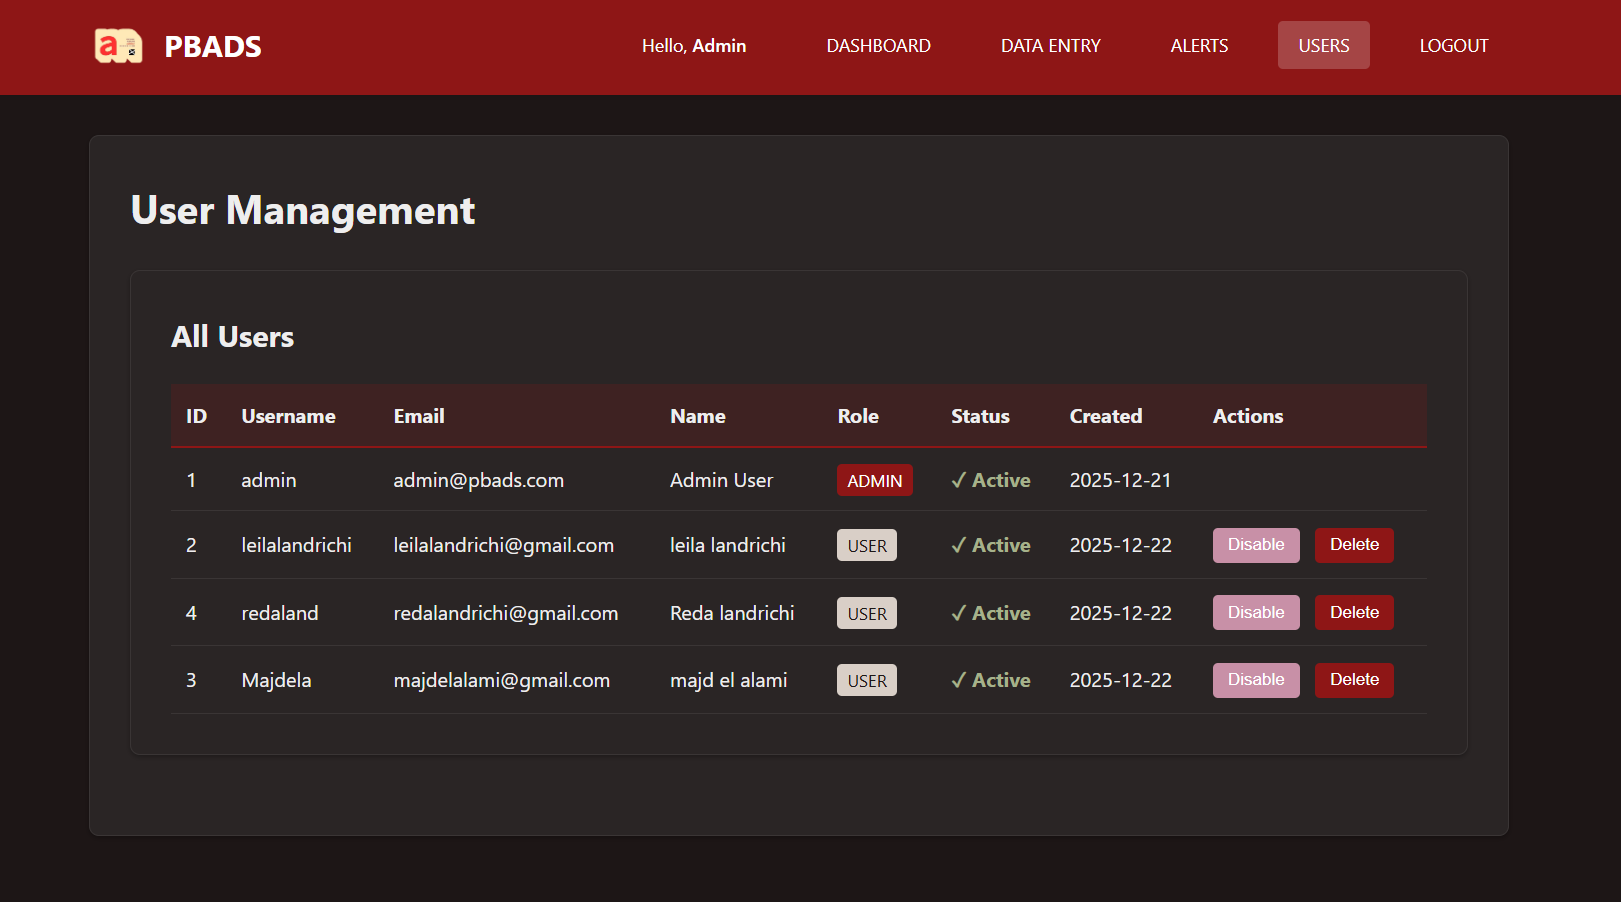
\includegraphics[width=\textwidth]{Figures/pbadsadmin/usermanagement.png}
    \caption{Interface de gestion des utilisateurs (Administrateur)}
    \label{fig:admin-user-management}
\end{figure}

Cette interface permet à l'administrateur de gérer tous les utilisateurs du système. Les fonctionnalités incluent :

\begin{itemize}
    \item \textbf{Liste complète des utilisateurs :} Affichage de tous les comptes utilisateurs
    \item \textbf{Opérations CRUD :} Création, lecture, mise à jour et suppression d'utilisateurs
    \item \textbf{Gestion des rôles :} Attribution des rôles ADMIN ou USER
    \item \textbf{Activation/Désactivation :} Contrôle de l'état actif/inactif des comptes
    \item \textbf{Informations détaillées :} Affichage des données utilisateur (nom d'utilisateur, email, rôle, statut)
    \item \textbf{Interface moderne :} Tableau responsive avec actions rapides
\end{itemize}

L'administrateur hérite de toutes les fonctionnalités utilisateur (tableau de bord, saisie de données, consultation des alertes) en plus de ces fonctionnalités de gestion.

\section{Conclusion}

Ce chapitre a présenté l'implémentation technique complète du système PBADS, couvrant l'architecture microservices, les technologies utilisées, et les interfaces développées pour les utilisateurs et les administrateurs.

L'architecture technique choisie, basée sur Spring Boot et Thymeleaf, offre une base solide et moderne pour le développement d'APIs REST robustes et performantes. L'utilisation de PostgreSQL avec JPA/Hibernate garantit une gestion efficace des données, tandis que l'intégration Kafka assure la communication asynchrone entre services. L'authentification JWT et le contrôle d'accès basé sur les rôles assurent une sécurité renforcée.

Les interfaces développées privilégient l'expérience utilisateur avec un thème sombre moderne, des graphiques interactifs avec Chart.js, et un système de notifications push en temps réel. Chaque rôle dispose d'interfaces adaptées à ses besoins spécifiques, facilitant ainsi l'adoption et l'efficacité du système.

Cette approche modulaire facilite la maintenance, l'évolution et l'adaptation de la solution aux besoins changeants, tout en garantissant une implémentation cohérente et robuste du système PBADS.
